\documentclass[english]{SPFShortReport}
\usepackage{subfigure}
\usepackage{spfFigures}
\usepackage{longtable}
\usepackage{url}
\usepackage{gensymb}
\usepackage[yyyymmdd,hhmmss]{datetime}
\reportName{Python calculation for heat pump SIN-30TE}
\reportSubName{Parametric Heat Pump calculation} 
\reportDate{\today \hspace{0.1cm} at: \currenttime \hspace{0.1cm} h} 
\author{Dani Carbonell}
\address{dani.carbonell@solarenergy.ch}
\begin{document}
\begin{table}[!ht]
\begin{small}
\caption{Fitted coefficients for the heat pump.}
\begin{center}
\resizebox{12cm}{!} 
{
\begin{tabular}{l | c c } 
\hline
\hline
Coefficient &Description & \\ 
 & &$[kW]$\\ 
\hline
$PQ_{1}$ & \emph{$1^{st}$ condenser polynomial coefficient}  & 2.7878e+01    \\ 
$PQ_{2}$ & \emph{$2^{st}$ condenser polynomial coefficient}  & 2.9731e+02    \\ 
$PQ_{3}$ & \emph{$3^{st}$ condenser polynomial coefficient}  & 9.2128e+01    \\ 
$PQ_{4}$ & \emph{$4^{st}$ condenser polynomial coefficient}  & -4.5257e+02    \\ 
$PQ_{5}$ & \emph{$5^{st}$ condenser polynomial coefficient}  & 4.0830e+02    \\ 
$PQ_{6}$ & \emph{$6^{st}$ condenser polynomial coefficient}  & -4.5471e+02    \\ 
\hline
$PCOP_{1}$ & \emph{$1^{st}$ COP polynomial coefficient}  & 5.9269e+00    \\ 
$PCOP_{2}$ & \emph{$2^{st}$ COP polynomial coefficient}  & 5.4679e+01    \\ 
$PCOP_{3}$ & \emph{$3^{st}$ COP polynomial coefficient}  & -2.8169e+00    \\ 
$PCOP_{4}$ & \emph{$4^{st}$ COP polynomial coefficient}  & -2.0992e+02    \\ 
$PCOP_{5}$ & \emph{$5^{st}$ COP polynomial coefficient}  & -2.0439e+00    \\ 
$PCOP_{6}$ & \emph{$6^{st}$ COP polynomial coefficient}  & -7.3062e+01    \\ 
\hline
$\dot m_{cond}$ & 5000.00 $[kg/h]$\\ 
$\dot m_{evap}$ & 5000.00 $[kg/h]$\\ 
\hline
$COP_{nom}$ (B0W35)& 4.32 \\ 
$Q_{c,nom}$ (B0W35)& 30.47 kW\\ 
$COP_{nom}$ (B2W35)& 4.54 \\ 
$Q_{c,nom}$ (B2W35)& 32.10 kW\\ 
$COP_{nom}$ (B10W35)& 5.40 \\ 
$Q_{c,nom}$ (B10W35)& 38.99 kW\\ 
\hline
\hline
\end{tabular}
}
\label{CoefTable}
\end{center}
\end{small}
\end{table}
\begin{table}[!ht]
\begin{small}
\caption{Predicting results of the heat pump.}
\begin{center}
\resizebox{12cm}{!} 
{
\begin{tabular}{l | c c c c c c c c c c c } 
\hline
\hline
$T_{evap,in}$ &$T_{evap,out}$ &$T_{cond,in}$ &$T_{cond,out}$ &$COP$ &$Q_{cond}$ &$Q_{evap}$ &$W_{comp}$ &$\dot m_{cond}$ &$\dot m_{evap}$ &$\Delta T_{evap}$ &$\Delta T_{cond}$ \\ 
$^oC$ &$^oC$ &$^oC$ &$^oC$ &$[-]$ &$[kW]$ &$[kW]$ &$[kW]$ &kg/h &kg/h &K &K\\ 
\hline
-7.00 & -10.47 & 25.72 & 30.00 & 3.81 & 24.93 & 18.39 & 6.54 & 5000 & 5000 & 3.5 & 4.3\\ 
-7.00 & -10.32 & 34.46 & 38.75 & 3.39 & 24.96 & 17.61 & 7.36 & 5000 & 5000 & 3.3 & 4.3\\ 
-7.00 & -9.94 & 43.35 & 47.50 & 2.82 & 24.13 & 15.58 & 8.55 & 5000 & 5000 & 2.9 & 4.1\\ 
-7.00 & -9.21 & 52.40 & 56.25 & 2.09 & 22.42 & 11.70 & 10.72 & 5000 & 5000 & 2.2 & 3.9\\ 
-7.00 & -7.60 & 61.57 & 65.00 & 1.19 & 19.96 & 3.18 & 16.78 & 5000 & 5000 & 0.6 & 3.4\\ 
-4.00 & -7.91 & 25.32 & 30.00 & 4.16 & 27.26 & 20.71 & 6.55 & 5000 & 5000 & 3.9 & 4.7\\ 
-4.00 & -7.73 & 34.08 & 38.75 & 3.68 & 27.18 & 19.79 & 7.39 & 5000 & 5000 & 3.7 & 4.7\\ 
-4.00 & -7.32 & 42.99 & 47.50 & 3.04 & 26.23 & 17.61 & 8.62 & 5000 & 5000 & 3.3 & 4.5\\ 
-4.00 & -6.55 & 52.05 & 56.25 & 2.24 & 24.41 & 13.53 & 10.88 & 5000 & 5000 & 2.6 & 4.2\\ 
-4.00 & -4.89 & 61.24 & 65.00 & 1.27 & 21.86 & 4.69 & 17.17 & 5000 & 5000 & 0.9 & 3.8\\ 
-1.00 & -5.36 & 24.90 & 30.00 & 4.51 & 29.67 & 23.10 & 6.57 & 5000 & 5000 & 4.4 & 5.1\\ 
-1.00 & -5.16 & 33.68 & 38.75 & 3.97 & 29.48 & 22.04 & 7.43 & 5000 & 5000 & 4.2 & 5.1\\ 
-1.00 & -4.72 & 42.62 & 47.50 & 3.26 & 28.42 & 19.71 & 8.71 & 5000 & 5000 & 3.7 & 4.9\\ 
-1.00 & -3.91 & 51.70 & 56.25 & 2.40 & 26.49 & 15.45 & 11.04 & 5000 & 5000 & 2.9 & 4.6\\ 
-1.00 & -2.19 & 60.90 & 65.00 & 1.36 & 23.85 & 6.31 & 17.53 & 5000 & 5000 & 1.2 & 4.1\\ 
2.00 & -2.82 & 24.47 & 30.00 & 4.87 & 32.16 & 25.56 & 6.61 & 5000 & 5000 & 4.8 & 5.5\\ 
2.00 & -2.60 & 33.28 & 38.75 & 4.26 & 31.86 & 24.37 & 7.49 & 5000 & 5000 & 4.6 & 5.5\\ 
2.00 & -2.13 & 42.23 & 47.50 & 3.49 & 30.69 & 21.89 & 8.80 & 5000 & 5000 & 4.1 & 5.3\\ 
2.00 & -1.29 & 51.33 & 56.25 & 2.56 & 28.66 & 17.45 & 11.21 & 5000 & 5000 & 3.3 & 4.9\\ 
2.00 & 0.48 & 60.55 & 65.00 & 1.45 & 25.92 & 8.05 & 17.88 & 5000 & 5000 & 1.5 & 4.5\\ 
5.00 & -0.30 & 24.03 & 30.00 & 5.23 & 34.74 & 28.10 & 6.65 & 5000 & 5000 & 5.3 & 6.0\\ 
5.00 & -0.05 & 32.85 & 38.75 & 4.55 & 34.33 & 26.78 & 7.55 & 5000 & 5000 & 5.1 & 5.9\\ 
5.00 & 0.44 & 41.82 & 47.50 & 3.72 & 33.05 & 24.16 & 8.89 & 5000 & 5000 & 4.6 & 5.7\\ 
5.00 & 1.31 & 50.94 & 56.25 & 2.72 & 30.91 & 19.54 & 11.38 & 5000 & 5000 & 3.7 & 5.3\\ 
5.00 & 3.13 & 60.17 & 65.00 & 1.54 & 28.09 & 9.89 & 18.20 & 5000 & 5000 & 1.9 & 4.8\\ 
8.00 & 2.21 & 23.57 & 30.00 & 5.58 & 37.41 & 30.71 & 6.70 & 5000 & 5000 & 5.8 & 6.4\\ 
8.00 & 2.48 & 32.41 & 38.75 & 4.84 & 36.88 & 29.27 & 7.62 & 5000 & 5000 & 5.5 & 6.3\\ 
8.00 & 3.00 & 41.40 & 47.50 & 3.95 & 35.50 & 26.50 & 9.00 & 5000 & 5000 & 5.0 & 6.1\\ 
8.00 & 3.90 & 50.54 & 56.25 & 2.88 & 33.26 & 21.71 & 11.54 & 5000 & 5000 & 4.1 & 5.7\\ 
8.00 & 5.77 & 59.79 & 65.00 & 1.64 & 30.34 & 11.84 & 18.51 & 5000 & 5000 & 2.2 & 5.2\\ 
11.00 & 4.70 & 23.10 & 30.00 & 5.95 & 40.15 & 33.40 & 6.75 & 5000 & 5000 & 6.3 & 6.9\\ 
11.00 & 4.99 & 31.96 & 38.75 & 5.14 & 39.52 & 31.84 & 7.69 & 5000 & 5000 & 6.0 & 6.8\\ 
11.00 & 5.54 & 40.96 & 47.50 & 4.18 & 38.03 & 28.93 & 9.10 & 5000 & 5000 & 5.5 & 6.5\\ 
11.00 & 6.48 & 50.12 & 56.25 & 3.05 & 35.69 & 23.98 & 11.71 & 5000 & 5000 & 4.5 & 6.1\\ 
11.00 & 8.38 & 59.38 & 65.00 & 1.74 & 32.69 & 13.90 & 18.79 & 5000 & 5000 & 2.6 & 5.6\\ 
14.00 & 7.18 & 22.61 & 30.00 & 6.31 & 42.98 & 36.17 & 6.81 & 5000 & 5000 & 6.8 & 7.4\\ 
14.00 & 7.49 & 31.49 & 38.75 & 5.44 & 42.25 & 34.48 & 7.76 & 5000 & 5000 & 6.5 & 7.3\\ 
14.00 & 8.07 & 40.52 & 47.50 & 4.42 & 40.65 & 31.44 & 9.21 & 5000 & 5000 & 5.9 & 7.0\\ 
14.00 & 9.03 & 49.68 & 56.25 & 3.22 & 38.20 & 26.34 & 11.87 & 5000 & 5000 & 5.0 & 6.6\\ 
14.00 & 10.97 & 58.97 & 65.00 & 1.84 & 35.12 & 16.07 & 19.05 & 5000 & 5000 & 3.0 & 6.0\\ 
17.00 & 9.64 & 22.11 & 30.00 & 6.68 & 45.89 & 39.02 & 6.87 & 5000 & 5000 & 7.4 & 7.9\\ 
17.00 & 9.98 & 31.01 & 38.75 & 5.75 & 45.05 & 37.21 & 7.84 & 5000 & 5000 & 7.0 & 7.7\\ 
17.00 & 10.58 & 40.05 & 47.50 & 4.66 & 43.35 & 34.04 & 9.31 & 5000 & 5000 & 6.4 & 7.4\\ 
17.00 & 11.57 & 49.24 & 56.25 & 3.39 & 40.81 & 28.78 & 12.03 & 5000 & 5000 & 5.4 & 7.0\\ 
17.00 & 13.54 & 58.53 & 65.00 & 1.95 & 37.64 & 18.34 & 19.29 & 5000 & 5000 & 3.5 & 6.5\\ 
20.00 & 12.09 & 21.60 & 30.00 & 7.05 & 48.88 & 41.95 & 6.93 & 5000 & 5000 & 7.9 & 8.4\\ 
20.00 & 12.45 & 30.51 & 38.75 & 6.06 & 47.94 & 40.02 & 7.92 & 5000 & 5000 & 7.6 & 8.2\\ 
20.00 & 13.07 & 39.57 & 47.50 & 4.90 & 46.14 & 36.72 & 9.42 & 5000 & 5000 & 6.9 & 7.9\\ 
20.00 & 14.09 & 48.78 & 56.25 & 3.57 & 43.50 & 31.32 & 12.18 & 5000 & 5000 & 5.9 & 7.5\\ 
20.00 & 16.09 & 58.09 & 65.00 & 2.06 & 40.24 & 20.73 & 19.51 & 5000 & 5000 & 3.9 & 6.9\\ 
\hline
\hline
\end{tabular}
}
\label{ResultsTable}
\end{center}
\end{small}
\end{table}
\begin{figure}[!ht]
\begin{center}
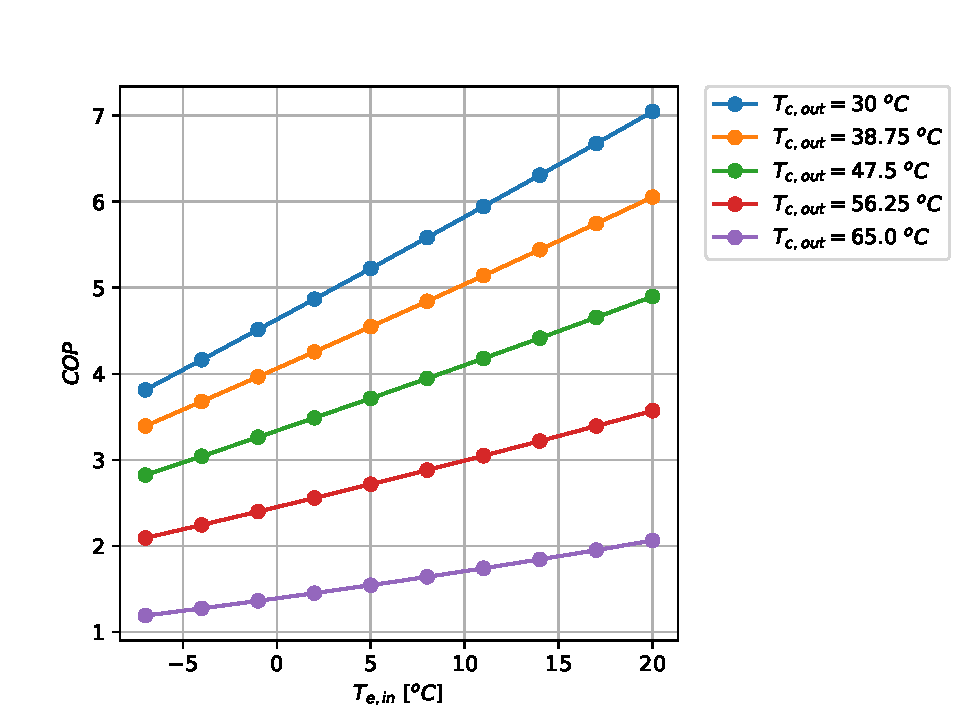
\includegraphics[width=1\textwidth]{C:/Daten/spfPackages/GIT/spfTrnsysFiles/HeatPump/BrineToWater/Walter Meier/SIN-30TE/SIN-30TE-Cop.pdf}
\caption{COP Results for the heat pump at the selected points}
\label{COPFig}
\end{center}
\end{figure}
\begin{figure}[!ht]
\begin{center}
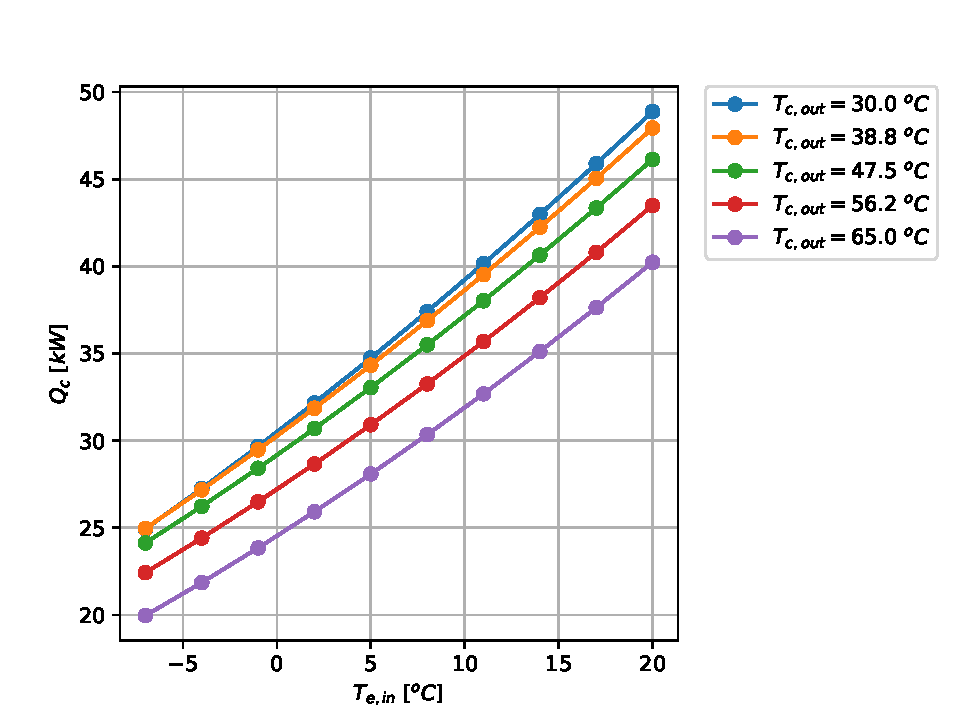
\includegraphics[width=1\textwidth]{C:/Daten/spfPackages/GIT/spfTrnsysFiles/HeatPump/BrineToWater/Walter Meier/SIN-30TE/SIN-30TE-Qc.pdf}
\caption{$Q_c$ Results for the heat pump at the selected points}
\label{QcFig}
\end{center}
\end{figure}
\end{document}
